\documentclass[conference,compsoc,11pt]{IEEEtran}


% *** CITATION PACKAGES ***
%
\ifCLASSOPTIONcompsoc
  \usepackage[nocompress]{cite}
\else
  \usepackage{cite}
\fi

% *** GRAPHICS RELATED PACKAGES ***
%
\ifCLASSINFOpdf
\else
\fi

%\hyphenation{op-tical net-works semi-conduc-tor}
\usepackage{graphicx}
\graphicspath{ {../img/} }


\begin{document}
\title{Convolutional Neural Network:\\ Plants Classification
\\ \large Artificial Neural Networks and Deep Learning -- a.y. 2022/2023}


\author{\IEEEauthorblockN{Paolo Botta\IEEEauthorrefmark{1},
Teo Bucci\IEEEauthorrefmark{2} and Silvia Caresana\IEEEauthorrefmark{3}}
\IEEEauthorblockA{M.Sc. Mathematical Engineering,
Politecnico di Milano - Milan, Italy\\
Email: \IEEEauthorrefmark{1}paolo.botta@mail.polimi.it,
\IEEEauthorrefmark{2}teo.bucci@mail.polimi.it,
\IEEEauthorrefmark{3}silvia.caresana@mail.polimi.it\\
Student ID: \IEEEauthorrefmark{1}10612869,
\IEEEauthorrefmark{2}10621873,
\IEEEauthorrefmark{3}10630163\\
Codalab Group: ``Just3Neurons''}
}
\maketitle


%\author{\IEEEauthorblockN{\textbf{Paolo Botta}}
%\IEEEauthorblockA{M.Sc. Computer Science and Engineering\\
%Politecnico di Milano - Milan, Italy \\
%E-mail: fabio1.tresoldi@mail.polimi.it \\
%Student ID : 10607540 \\
%Codalab Nickname: "fabioow" \\
%Codalab Group: "artificial\_comrades"}
%\and
%\IEEEauthorblockN{\textbf{Teo Bucci}}
%\IEEEauthorblockA{M.Sc. Computer Science and Engineering\\
%Politecnico di Milano - Milan, Italy \\
%E-mail: mirko.usuelli@mail.polimi.it \\
%Student ID : 10570238 \\
%Codalab Nickname: "mirko" \\
%Codalab Group: "artificial\_comrades"}
%\and
%\IEEEauthorblockN{\textbf{Teoasd Bucci}}
%\IEEEauthorblockA{M.Sc. Computer Science and Engineering\\
%Politecnico di Milano - Milan, Italy \\
%E-mail: mirko.usuelli@mail.polimi.it \\
%Student ID : 10570238 \\
%Codalab Nickname: "asdasd" \\
%Codalab Group: "artificial\_comrades"}}

\maketitle

\begin{abstract}
TODO%In this report, we explore and compare the development process we had to design a Convolutional Neural Network able to classify 14 different plants species through their leaves images as input.
\end{abstract}
\IEEEpeerreviewmaketitle

\section{Introduction}
The given dataset consists of 3542 images belonging to 8 different classes. To build the classifier, many choices about the model had to be made. Since the settings that can be tweaked in the model would generate many more configurations than our computational power could handle, we followed an incremental approach. Specifically, we started with a baseline and slowly made choices from there, seeing whether the performance improved or not, trying to understand why and if the outcome was expected.

The task suggests to use Categorical Crossentropy as loss function, and as metric we used Accuracy as requested. In addition, we also considered the F1-score per class to better understand the weaknesses of the model.

The dataset was split according to an 85:15 train-validation ratio and the results of this report are the ones we obtained on the validation set. We chose this ratio because since the dataset was quite small for the task we wanted to take advantage of all the information possible.


\begin{figure}[h!]
\centering
%\includegraphics[width=1.9in]{img/development.png}
\caption{Development Process.}
\label{fig_sim}
\end{figure}

\section{Data Pipeline}
\subsection{Data Augmentation}
Since the dataset is not very numerous, Data Augmentation was used almost from the beginning in all models, allowing the network to better generalize and have a better performance. We used Traditional Transformations: Rotating, Zooming, Flipping, Brightness, Shifting, Shear.
Initially only the first three were used, but adding all of them showed an increase of 1-2\% in accuracy.\\
We thought of using also more advanced transformations like CutMix or CutOut, but given that the dataset is made of plants more or less homogeneous in each sample, we discarded those options and focused our attention more on the architecture for the time being.

%\subsubsection{Traditional Transformations}
%Rotating, Zooming, Flipping, Brightness, Shifting.
%\subsubsection{Advanced Transformations}
%CutMix, MixUp, CutOut.

%However, these last Advance Transformations did not increased the overall performance in our specific case, but indeed, they made the training process slower and not as accurate as without them, therefore we decided to discard these techniques.

%In terms of validation accuracy, within 20 epochs:

\begin{center}
\begin{tabular}{ c c }
\hline\hline
 No Augmentation & 99.86\% \\ 
\hline
 Traditional Transf. & \textbf{99.93\%}  \\  
 Advanced Transf. & 99.79\% \\
\hline\hline
\end{tabular}
\end{center}

\begin{figure}[h!]
\centering
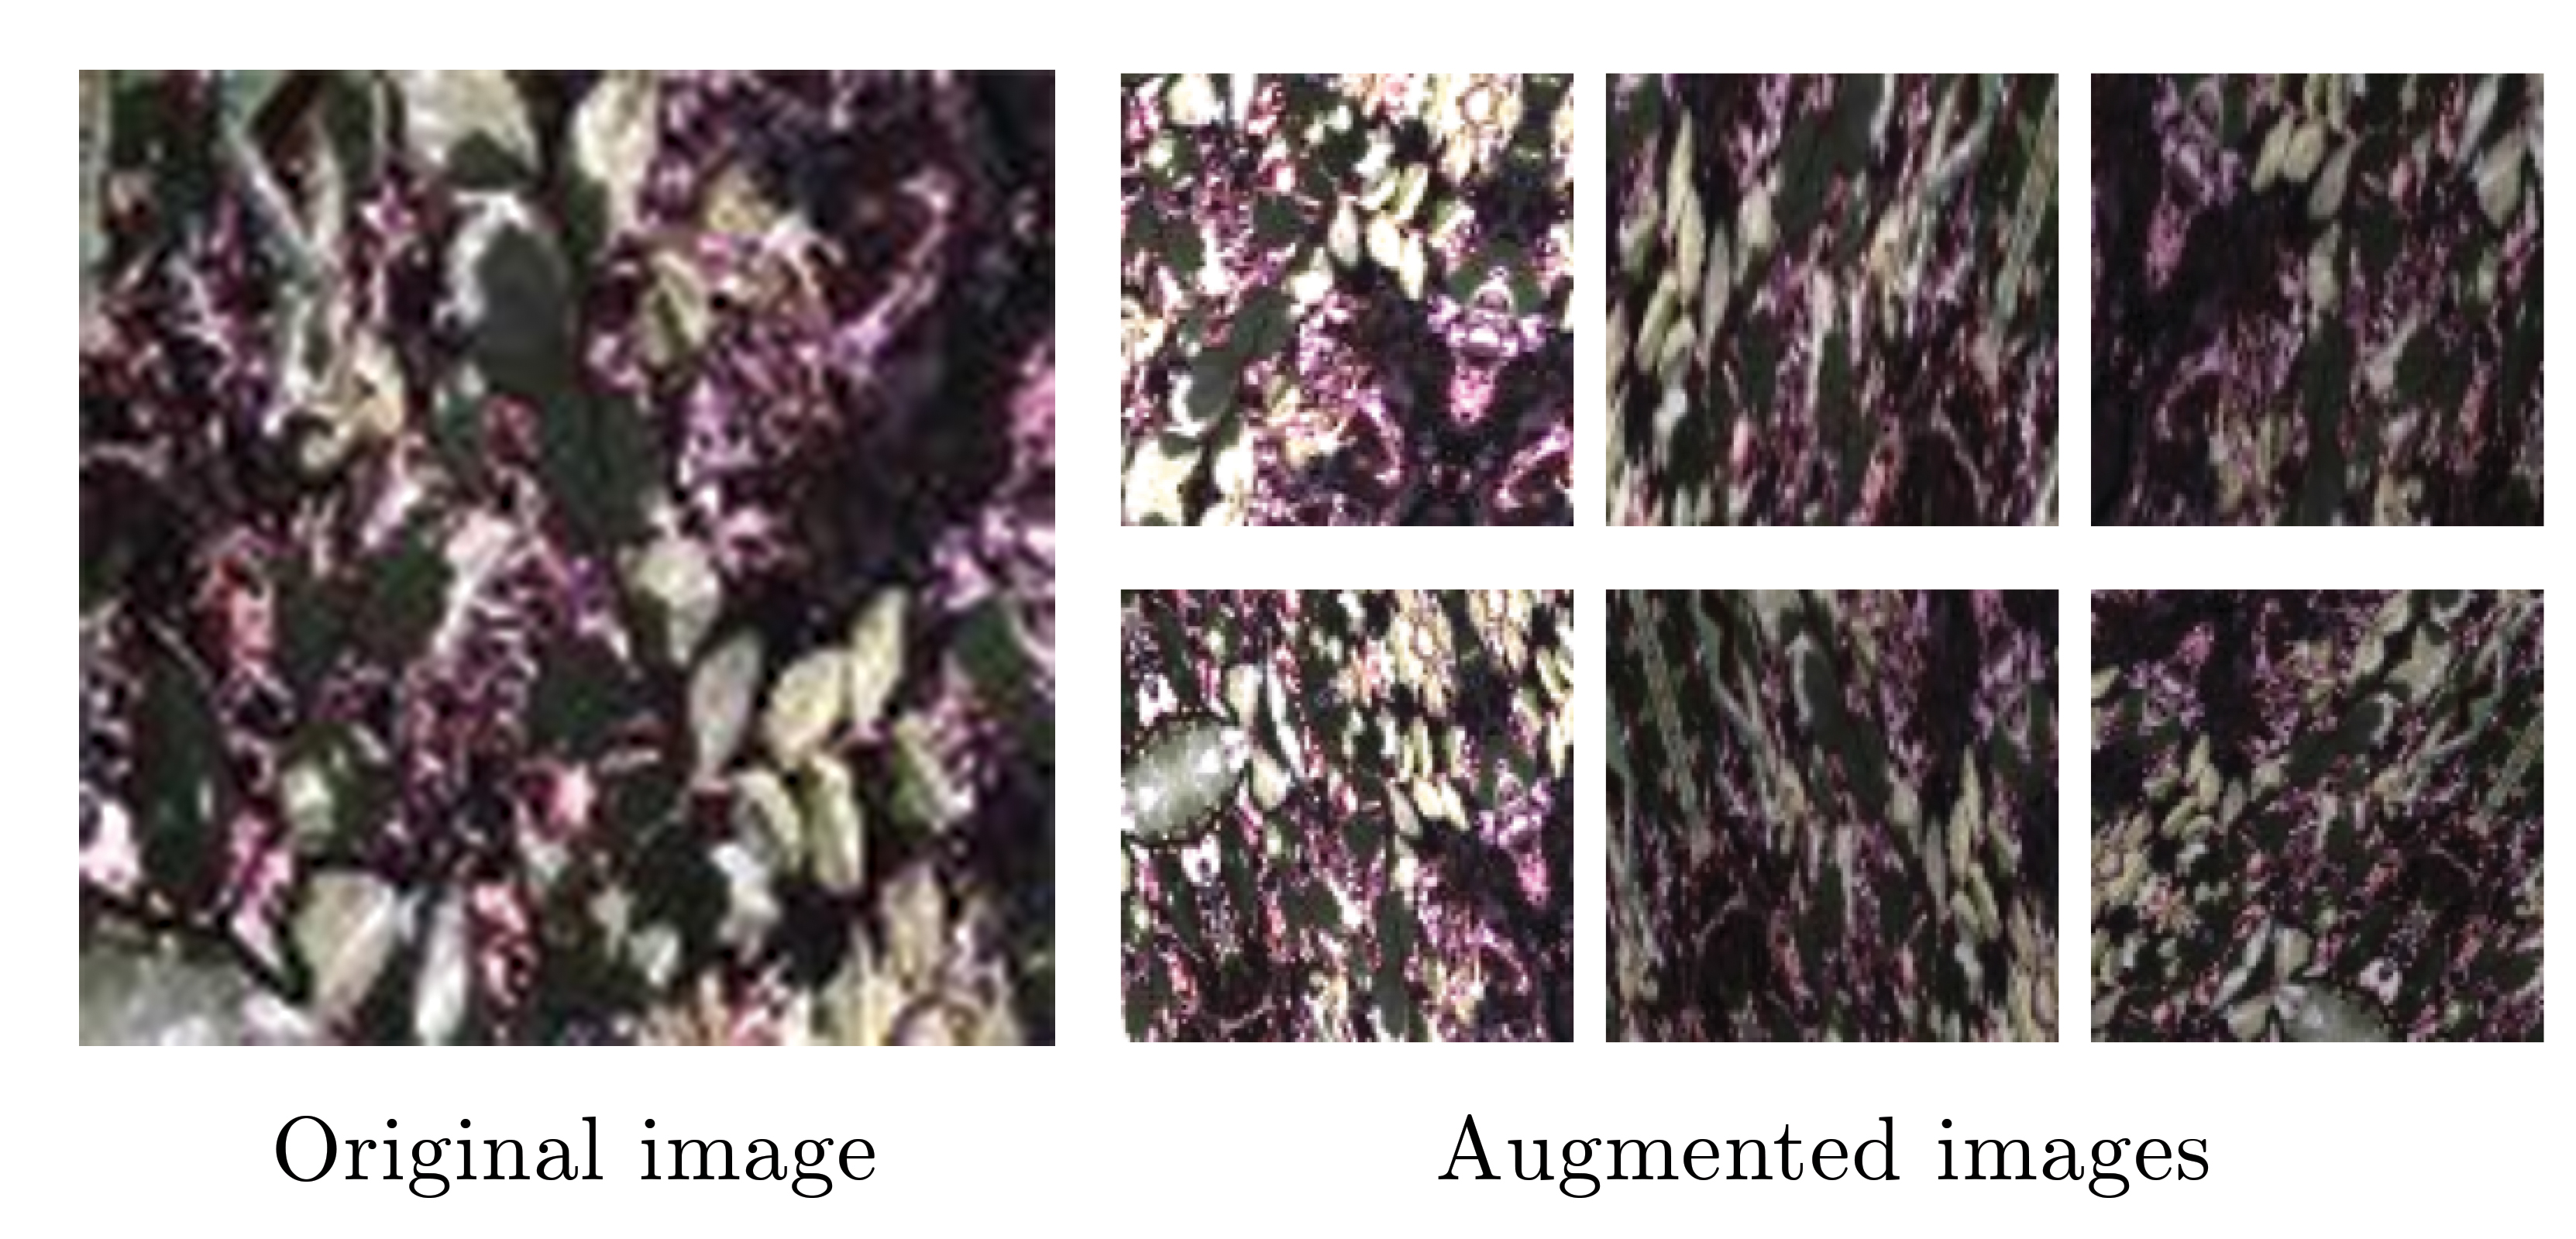
\includegraphics[width=3.1in]{single_augmentation.jpg}
\caption{Some examples of Data Augmentation techniques.}
\label{fig_sim}
\end{figure}

\subsection{Pre-Processing}
According to the documentation, the Features Extractor (see section \ref{sec:features-extractor}) that we chose works best with standardized inputs. Therefore, data processing was done according to the \verb|preprocess_input| contained in \verb|tensorflow.keras.applications|.
%Since for the Features Exctractor (section 3.1) we relied on State-of-Art architectures through Fine Tuning, the data pre-processing function adopted is the same suggested by the corresponding model contained in \texttt{tensorflow.keras.applications}.

\section{Convolutional Neural Network}
We started with a baseline model adopting the classical architecture of modern CNNs using 5 blocks of \verb|Conv2D| + \verb|MaxPooling2D| and a \verb|Dense| layer with 512 neurons, obtaining a starting accuracy of 54.67\%.
Then we turned to some pre-trained models to perform transfer learning. Given the reduced size of the dataset we were quite sure this would greatly cut training time.

\subsection{Features Extractor}\label{sec:features-extractor}
To choose our features extractor we compared some famous architectures equipped with a simple classifier of 512 neurons and run the simulation for 30 epochs.

\begin{figure}[h!]
\centering
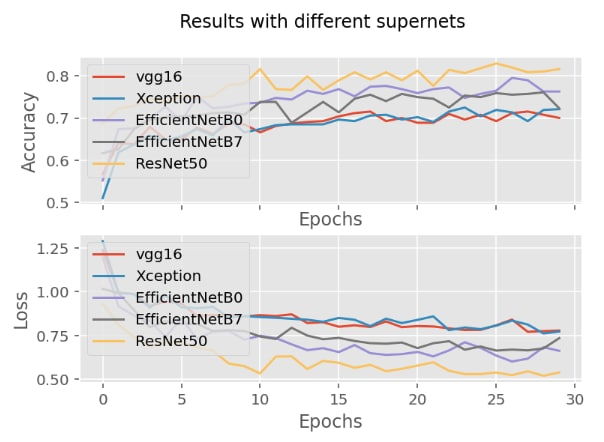
\includegraphics[width=3.1in]{supernet.jpg}
\caption{State-of-Art architectures comparison.}
\label{fig_sim}
\end{figure}

According to the results in Figure \ref{fig_sim}, the best model was ResNet50. However, we decided to keep both that and VGG16 given its fast inference time.

\begin{center}
\begin{tabular}{ l c }
\hline\hline
Xception & 68.31\% \\
EfficientnetB0 & 77.23\% \\
EfficientnetB7 & 73.24\% \\
Resnet50 & \textbf{79.51}\% \\
VGG16 & 68.69\% \\
\hline\hline
\end{tabular}
\end{center}

% \subsubsection{Ensemble}
% Then we started introducing the concept of Ensemble in order to reduce the overall variance in prediction. By taking the input multiple times through different Features Extractors, we concatenated the GAP ouput for each model in purpose to feed the final classifier with different conclusions.

% \begin{figure}[h!]
% \centering
% \includegraphics[width=2.5in]{img/ensemble.png}
% \caption{CNN Ensemble.}
% \label{fig_sim}
% \end{figure}

% However, this method performed worse than a single CNN, therefore we discarded this technique.

% \begin{center}
% \begin{tabular}{ c c }
% \hline\hline
%  EfficientNetB0 & \textbf{99.97\%}  \\  
%  EfficientNetB0+B1 & 99.92\%  \\
%  EfficientNetB0+B1+B2 & 99.88\% \\
% \hline\hline
% \end{tabular}
% \end{center}

\subsection{Classifier}
Starting from a general classifier model, with the main layers shown during the course, we analyzed the performance of each of them through Transfer Learning:

% \begin{figure}[h!]
% \centering
% \includegraphics[width=3.3in]{img/classifier.png}
% \caption{Baseline Classifier Architecture.}
% \label{fig_sim}
% \end{figure}

\subsubsection{Global Average Pooling Layer} After the convolutional base we initially had a Flatten layer, which we later switched to GlobalAveragePooling2D to better summarize the output of the feature extractor. The improvements weren't significant, yet there was a reduction in the number of parameters and in training time.


DENSE LAYER STUFF

% \subsubsection{Dense Layer} The sizes we tested for the dense layer were:
% \begin{center}
% \begin{tabular}{ c c }
% \hline\hline
%  0 (only GAP) & 98.89\% \\ 
% \hline
%  64 neurons & 98.79\%  \\  
%  128 neurons & 98.87\%  \\
%  256 neurons & \textbf{98.90\%} \\
%  512 neurons & 98.79\%\\
% \hline
%  256 neurons (x2) & 98.89\%  \\  
% \hline\hline
% \end{tabular}
% \end{center}

TODO SISTEMARE Batch Normalization: improve training time and accuracy by 1-2%

%\subsubsection{Batch Normalization Layer} We introduced the batch normalization in order to have learnable parameters to be used for the regularization process.

% \subsubsection{Activation Function Layer} We took into account the main three CNN activation functions in order to find the best matching one:
% \begin{center}
% \begin{tabular}{ c c }
% \hline\hline
%  ReLU & \textbf{98.87\%}  \\  
%  LeakyReLU & 98.73\%  \\
%  GeLU & 98.14\% \\
% \hline\hline
% \end{tabular}
% \end{center}

% \subsubsection{DropOut Layer} We tried DropOut as boosting technique; the hyperparameters we tested were:
% \begin{center}
% \begin{tabular}{ c c }
% \hline\hline
%  No DropOut & \textbf{98.93\%} \\ 
% \hline
%  DropOut(0.1) & 98.84\%  \\  
%  DropOut(0.2) & 98.87\%  \\
%  DropOut(0.3) & 98.86\% \\
% \hline\hline
% \end{tabular}
% \end{center}

\subsubsection{Dropout} Dropout was always used after the Dense layer for regularization, to the point that sometimes the validation accuracy was higher than training, significantly highlighting the generalization of the model.


\section{Training techniques}

Initially, transfer learning was performed first by training the classifier with the convolutional base frozen, and then tuning with a lower learning rate with the last 4 layers of VGG16 unfrozen. However, we noticed that the performance barely reached 75\%, so we decided to introduce the idea of \textbf{multiple passes}. We thought that the latent representation of the last frozen layers of VGG16 wasn't still in line with our dataset, so progressively we unfroze more layers and did more fine-tuning with an even lower learning rate until all layers but the first three were trainable.
This gave a great improvement, about 10-11\% more accuracy. TODO METTI TABLE

TODO riscrivere
Another idea, which let us reach 0.9050 in our validation, was to address the class imbalance. Oversampling the dataset didn’t seem to be the most elegant solution, so we decided to compute the class weights according to the number of samples (less represented classes had a higher weight) and passed it to the fit() command. This led to a weighted loss function that gave more weight to the less represented classes when performing backpropagation. As expected, F1 scores for such classes saw an improvement of about 10-15%.
Strangely enough, 0.905 was reached only specifying class weights during the first transfer learning pass, and was lower when specifying it also in the final passes.




\section{Conclusion}

TODO FARE CONCLUSIONI

Final Model
The final model was built by choosing
batch size 16
loss: CategoricalCrossEntropy
optimizer: TODO
Numbero unfrozen layer from the last: 4,8,12,15

[summary modello con numero parametri e trainable]


Performance
The model, trained with EarlyStopping with patience 15 based on validation accuracy, got the following results:

train loss train acc val loss val acc
tabella


Confusion Matrix
We evaluated the confusion matrix on the [TRAIN O VALIDATION] reaching the following indexes

f1 per ogni cosa
confusion matrix
accuracy


ReduceLRonPlaeaut callback da qualche parte



Further Developments
We acknowledge that our workflow might use some more procedure, however, having at our disposal limited resources, the trial and error approach seemed to be best. We are satisfied with the results, while possible room for improvement could be to use some more advanced augmentation techniques to help the generalization power of the model, and try more advanced pretrained models. Moreover, we could experiment with different optimizers and learning rates.

% \subsection{Final Model}
% The final model setting submitted is: \\
% - \textbf{batch\_size} : 32 \\
% - \textbf{loss} : Categorical Crossentropy \\
% - \textbf{optimizer} : Adam(1e-4) \\
% - \textbf{fine\_tuning\_layer} : 162 (\texttt{block6a\_expand\_conv})
% \begin{center}
% \begin{tabular}{ c | c c }
% \hline
%   \textbf{Layer (type)} & \textbf{Output Shape} & \textbf{Param #} \\ 
% \hline\hline
%  \texttt{input} & [(None, 256, 256, 3)] & 0  \\
%  \texttt{efficientnetb0} & (None, 8, 8, 1280) & 4049571  \\  
%  \texttt{global\_avg\_pool} & (None, 1280) & 0 \\
%  \texttt{dense} & (None, 256) & 327936 \\
%  \texttt{batch\_norm} & (None, 256) & 1024 \\
%  \texttt{re\_lu}  & (None, 256) & 0 \\
%  \texttt{softmax} & (None, 14) & 3598 \\
% \hline\hline
% \end{tabular}
% \end{center}
% \begin{center}
% \begin{tabular}{ c c }
% \textbf{Total params}: & 4,382,129 \\
% \textbf{Trainable params}: & 3,487,786 \\
% \textbf{Non-trainable params}: & 894,343 \\
% \hline
% \end{tabular}
% \end{center}

% \begin{figure}[h!]
% \centering
% \includegraphics[width=3.3in]{img/final.png}
% \caption{Final model architecture.}
% \label{fig_sim}
% \end{figure}

\subsection{Performance}
The dataset has been split in 80\% for training and 20\% for validation. The model in training, evaluated with an Early Stopping with patience 10 epochs based on validation loss, reached the peak of performance at epoch 34 with the following indexes:


TODO SISTEMARE QUA
\begin{center}
\begin{tabular}{ c c | c c }
\hline\hline
  \textbf{Train. loss} & \textbf{Train. acc.} & \textbf{Val. loss} & \textbf{Val. acc.}   \\ 
\hline
 0.0036 & 99.89\% & 0.0019 & 99.97\% \\  
\hline\hline
\end{tabular}
\end{center}

\subsection{Confusion Matrix}
Finally, we generated the confusion matrix to identify the correctness of classification for each class with F1-score, precision and recall, on the dataset split in 60\% for training and 20\% each for validation and testing. Testing set performance indexes:

\begin{itemize}
\item \textbf{Accuracy} : 99.77\%
\item \textbf{Precision} : 99.78\%
\item \textbf{Recall} : 99.75\%
\item \textbf{F1-score} : 99.76\%
\end{itemize}

TODO METTERE CONFUSION
% \begin{figure}[h!]
% \centering
% \includegraphics[width=3.5in]{img/confusion_matrix.png}
% \caption{Confusion Matrix on the Testing set.}
% \label{fig_sim}
% \end{figure}

% \subsection{Leadboard Evaluation}
% \begin{itemize}
% \item Development phase accuracy : \textbf{94.91\%}
% \item Final phase accuracy: \textbf{94.53\%}
% \end{itemize}

%\begin{thebibliography}{1}
%\bibitem{IEEEhowto:perez}
%L. Perez and J. Wang}, \emph{The Effectiveness %of Data Augmentation in Image Classification %using Deep Learning} - \relax Stanford %University, 2017.
%\end{thebibliography}

\end{document}